%% For double-blind review submission, w/o CCS and ACM Reference (max submission space)
% \documentclass[sigplan,10pt,review,anonymous]{acmart}\settopmatter{printfolios=true,printccs=false,printacmref=false}
%% For double-blind review submission, w/ CCS and ACM Reference
%\documentclass[acmsmall,review,anonymous]{acmart}\settopmatter{printfolios=true}
%% For single-blind review submission, w/o CCS and ACM Reference (max submission space)
%\documentclass[acmsmall,review]{acmart}\settopmatter{printfolios=true,printccs=false,printacmref=false}
%% For single-blind review submission, w/ CCS and ACM Reference
%\documentclass[acmsmall,review]{acmart}\settopmatter{printfolios=true}
%% For final camera-ready submission, w/ required CCS and ACM Reference
\documentclass[acmsmall,nonacm]{acmart}\settopmatter{}


%% Journal information
%% Supplied to authors by publisher for camera-ready submission;
%% use defaults for review submission.
\acmJournal{PACMPL}
\acmVolume{1}
\acmNumber{CONF} % CONF = POPL or ICFP or OOPSLA
\acmArticle{1}
\acmYear{2018}
\acmMonth{1}
\acmDOI{} % \acmDOI{10.1145/nnnnnnn.nnnnnnn}
\startPage{1}

%% Copyright information
%% Supplied to authors (based on authors' rights management selection;
%% see authors.acm.org) by publisher for camera-ready submission;
%% use 'none' for review submission.
\setcopyright{none}
%\setcopyright{acmcopyright}
%\setcopyright{acmlicensed}
%\setcopyright{rightsretained}
%\copyrightyear{2018}           %% If different from \acmYear

%% Bibliography style
\bibliographystyle{ACM-Reference-Format}
%% Citation style
%% Note: author/year citations are required for papers published as an
%% issue of PACMPL.
% \citestyle{acmauthoryear}   %% For author/year citations


%%%%%%%%%%%%%%%%%%%%%%%%%%%%%%%%%%%%%%%%%%%%%%%%%%%%%%%%%%%%%%%%%%%%%%
%% Note: Authors migrating a paper from PACMPL format to traditional
%% SIGPLAN proceedings format must update the '\documentclass' and
%% topmatter commands above; see 'acmart-sigplanproc-template.tex'.
%%%%%%%%%%%%%%%%%%%%%%%%%%%%%%%%%%%%%%%%%%%%%%%%%%%%%%%%%%%%%%%%%%%%%%


%% Some recommended packages.
\usepackage{booktabs}   %% For formal tables:
                        %% http://ctan.org/pkg/booktabs
\usepackage{subcaption} %% For complex figures with subfigures/subcaptions
                        %% http://ctan.org/pkg/subcaption
\usepackage{xcolor}
\usepackage{listings}
\lstset{
  basicstyle=\fontsize{8}{10}\selectfont\ttfamily,
  numbers=left,
  numberstyle= \tiny,
  keywordstyle= \color{ blue!70},
  commentstyle= \color{red!50!green!50!blue!50},
  frame=single,
  rulesepcolor= \color{ red!20!green!20!blue!20} ,
  escapeinside=``,
  xleftmargin=1.5em,xrightmargin=0em, aboveskip=1em,
  framexleftmargin=2em,
  showstringspaces=false,
  showtabs=false,
  breaklines=true
}
\lstdefinelanguage{Solidity}
{
  morekeywords={contract, mapping, address, uint, private, function, public, if, payable},
  morecomment=[l]{//},
  morestring=[b]"
}

% \usepackage{biblatex}

\usepackage{multicol}
\usepackage{lipsum}
\usepackage{mathtools}
\usepackage{cuted}

\usepackage{amsmath}
\usepackage{extpfeil}
\usepackage{mathpartir}
\usepackage[mathscr]{eucal}

\usepackage{caption}

\usepackage{hyperref}
\usepackage{cleveref}

% \usepackage[style=authoryear-comp]{biblatex}
% \DeclareLabeldate[online]{%
%   \field{date}
%   \field{year}
%   \field{eventdate}
%   \field{origdate}
%   \field{urldate}
% }
% \DeclareLabeldate{\field{date}\field{eventdate} \field{origdate}\literal{nodate}}

% \DefineBibliographyStrings{english}{%
% nodate = {\ifboolexpr{test{\ifentrytype{misc1}} or test{\ifentrytype{misc5}}}{}{o\adddot D\adddot}},
% }

\crefformat{section}{\S#2#1#3} % see manual of cleveref, section 8.2.1
\crefformat{subsection}{\S#2#1#3}
\crefformat{subsubsection}{\S#2#1#3}


\begin{document}

%% Title information
\title[]{CS222 Project Proposal}         %% [Short Title] is optional;
%% when present, will be used in
%% header instead of Full Title.

\author{Yichen Xie}
% \authornote{Supervised by Qinxiang Cao, Shanghai Jiao Tong University, John Hopcroft Center for Computer Science.}          %% \authornote is optional;
%% can be repeated if necessary
%\orcid{nnnn-nnnn-nnnn-nnnn}             %% \orcid is optional
\affiliation{
	%\position{Position2b}
	%\department{Department2b}             %% \department is recommended
	\institution{Shanghai Jiao Tong University}           %% \institution is required
	%\streetaddress{Street3b Address2b}
	%\city{City2b}
	%\state{State2b}
	%\postcode{Post-Code2b}
	%\country{Country2b}                   %% \country is recommended
}
% \email{}          %% \email is recommended

\author{Zhongye Wang}
% \authornote{Supervised by Qinxiang Cao, Shanghai Jiao Tong University, John Hopcroft Center for Computer Science.}          %% \authornote is optional;
%% can be repeated if necessary
%\orcid{nnnn-nnnn-nnnn-nnnn}             %% \orcid is optional
\affiliation{
	%\position{Position2b}
	%\department{Department2b}             %% \department is recommended
	\institution{Shanghai Jiao Tong University}           %% \institution is required
	%\streetaddress{Street3b Address2b}
	%\city{City2b}
	%\state{State2b}
	%\postcode{Post-Code2b}
	%\country{Country2b}                   %% \country is recommended
}
\email{wangzhongye1110@sjtu.edu.cn}          %% \email is recommended

\author{Xinyu Zhan}
% \authornote{Supervised by Qinxiang Cao, Shanghai Jiao Tong University, John Hopcroft Center for Computer Science.}          %% \authornote is optional;
%% can be repeated if necessary
%\orcid{nnnn-nnnn-nnnn-nnnn}             %% \orcid is optional
\affiliation{
	%\position{Position2b}
	%\department{Department2b}             %% \department is recommended
	\institution{Shanghai Jiao Tong University}           %% \institution is required
	%\streetaddress{Street3b Address2b}
	%\city{City2b}
	%\state{State2b}
	%\postcode{Post-Code2b}
	%\country{Country2b}                   %% \country is recommended
}
% \email{}          %% \email is recommended


% %% Abstract
% %% Note: \begin{abstract}...\end{abstract} environment must come
% %% before \maketitle command
% \begin{abstract}
% 	Text of abstract \ldots
% \end{abstract}


%% 2012 ACM Computing Classification System (CSS) concepts
%% Generate at 'http://dl.acm.org/ccs/ccs.cfm'.

%% End of generated code


%% Keywords
%% comma separated list
\keywords{}  %% \keywords are mandatory in final camera-ready submission


%% \maketitle
%% Note: \maketitle command must come after title commands, author
%% commands, abstract environment, Computing Classification System
%% environment and commands, and keywords command.
\maketitle

% xyc, until the last
\section{Introduction}
% Recent years have witnessed the rapid development of deep learning.
The development of deep learning has proved its great capability, and it will be more beneficial if we can plant deep learning models into edge devices like wearable devices.
However, the limited energy supply and computational capability of edge devices lead to constraints on the scale and complexity of deep neural networks.
We need light-weight models to meet these requirements of edge device.
In this project, we will seek for a combination of light-weight neural networks to substitute the original complex model while preserving its functionality.
% With this new model, we will try to reduce the parameter number and computing consumption notably at the expense of acceptable accuracy decline compared to the original large model.

% xyc
\section{Problem Description}
We mainly focus on the task to replace a large deep learning model with a set of small models with reduced complexity.
Using too many small models can still result in tremendous amount of calculation in inference and affect models' performance in edge devices, so we limit the overall complexity of models as well.
% Then, the total computational consumption can decrease definitely.
As a result, edge device can profit from the lowered demand for computational consumption.
% And these small models are independent from the original deep learning network at least in the inference phase.
% Hence, they can process the data on the edge device without communication with the cloud or servers, which extend the application range of these device.

There are many possible approaches in the design of small model system.
\begin{itemize}
  \item We could train small models each with specific tasks, which can be implemented with satisfying performance and simple network structure.
  \item We could train small models each dealing with part of the dataset, which can be combined to handle all data points efficiently.
\end{itemize}
Our focus will be the former one, where we want each model to perform binary decisions in the context of classification and the union of these models should uniquely determine the category of any sample.
In this way, small models serve as feature extractors that jointly produce an embedding for the data sample.
We can also retrieve such embedding implicitly using neural networks, but we choose to achieve the optimal embedding explicitly by solving the search problem formulated in \cref{sec:formulation}.

We will take the image recognition (classification) task as the example throughout the project.
At present, AdaBoost tends to be one possible solution.
However, the weaker learners in these algorithm, which may be very simple classifiers, are so susceptible that the outcome is sensitive to noisy data and outliers.
By contrast, thanks to the application of neural networks and more sophisticated combination methods, we will attempt to pursue a more robust and accurate model.

% wzy
\section{Problem Formulation}
\label{sec:formulation}
There has not been much time for us to fully consider the optimal way of addressing the problem, but we do propose one possible formulation and some solution ideas in this section.

Assume there are $N$ classes in total, each denoted by $A_i$.
We further divide each class $A_i$ into $M_i$ subsets $A_{ij}$ according to some features of samples, e.g., the activation of certain convolution filters.
Now, we have a set $\mathcal{D}$ of $K$ (a relatively large number) binary classifiers each identifying a subset of all $A_{ij}$ classes.
Say classifier $d$ separates $\{A_{ij} \,|\, (i, j) \in I_d\}$ from the rest of classes, i.e., given any sample, it determines wether the label of the sample belongs to $I_d$.
Here, $I_d$ is the positive label set defined by the classifier $d$.
Note that we can always define a compliment classifier whose positive label set is exactly the negative label set of the classifier $d$.

Our task is to find a subset $D^* \subset \mathcal{D}$, such that for any class $A_i$, there exists a partition that divides it into some subclasses $S_i^{(l)}$ where $A_i = \bigcup_l \{A_{ij} \,|\, (i, j) \in S_i^{(l)}\}$, and for each subclass $S_i^{(l)}$ there exists a subset of classifiers $D^{(l)} \subseteq D^*$ where $S_i^{(l)} = \bigcap_d \{I_d \,|\, d \in D^{(l)}\}$.
Here, subclass $S_i^{(l)}$ represents the union of some subsets $A_{ij}$ of class $A_i$, and the union of all subclasses of $A_i$ should reconstruct the $A_i$ itself.
The optimal set of classifiers $D^*$ should allow us to determine wether a sample belongs to any given subclass $S_i^{(l)}$ using a subset $D^{(l)}$ in it, which in turn determines wether the sample belongs to $A_i$.
Figure~\ref{fig:feasible-example} shows a feasible classifier set $D$ in a simple example.

\begin{figure}[h]
    \centering
    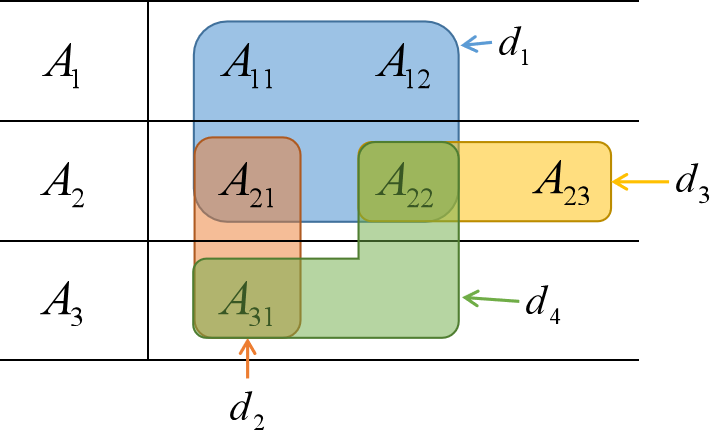
\includegraphics[width=0.45\linewidth]{fig/formulation_example.png}
    \caption{An Example of Feasible Classifier Set:
    The samples in class $A_1$ is further divided into $A_{11}, A_{12}$ and those in class $A_2$ is further divided into $A_{21}, A_{22}, A_{23}$.
    We do not divide $A_3$ but rename it to $A_{31}$.
    There are 4 discriminators $d_1, d_2, d_3, d_4$ respectively identify $\{A_{11}, A_{12}, A_{21}, A_{22}\}$, $\{A_{21}, A_{31}\}$, $\{A_{22}, A_{23}\}$, and $\{A_{23}, A_{31}\}$.
    We have: \textit{(a)} the intersection of $d_1$ and the compliments of $d_2, d_3$ identifies $A_1 = A_{11} \cup A_{12}$;
    \textit{(b)} the intersection of $d_1$ and $d_2$ identifies $A_{21}$, and its union with $d_3$ determines the entire $A_2$;
    \textit{(c)} the intersection of $d_3$ and the compliment of $d_1$ determines $A_3 = A_{31}$.
    Clearly, $D = \{d_1, d_2, d_3\}$ is a feasible set, where the redundant classifier $d_4$ is not selected.}
    \label{fig:feasible-example}
\end{figure}

There are further constraints and considerations of the optimal set of classifiers $D^*$.
\begin{itemize}
    \item \textbf{Number of Classifiers.} We need to choose adequate number of classifiers $|D^*|$ so that it covers all classes. But we prefer to use as less classifiers as possible to save computational consumptions.
    \item \textbf{Network Size.} The size of each classifier is limited. Large networks as classifiers improve accuracy but slow down inferences. Therefore, we will have penalty for large classifiers.
    \item \textbf{Overall Accuracy.} We know the accuracy of each classifier as a prior, but we need to derive the overall accuracy based on it. The $D^*$ should optimize the overall accuracy along with other goals.
\end{itemize}
These are factors we will consider in the later development and we are open for other suggestions.

Beside these factors, there are other implementation issues about the solution to the problem.
We have considered a given search space for small models, where the performance and functionality of each model is known as a prior.
This allows us to concentrate on the search part of the solution.
Nevertheless, we do not have such a prior in practice.
Instead, we need to determine the next small model to be explored during the search, which we could potentially formulate as a local search problem.

% zxy
\section{Related Work}
\paragraph{\textbf{Ensemble method}} 
Ensemble method solves the learning problem by combining several learners.
A few researchers have addressed the issue of combining a set of simple classifier. 
Beriman\cite{BreimanBagging} proposed a method for generating multiple versions of a predictor by making bootstrap replicates of the learning set. 
However, this method actually increased the amount of computation since it trained the learned repeatedly.
Schapire\cite{Schapire1989The} proposed the boosting method to converting a weak learning algorithm into one that achieves arbitrarily high accuracy by combining a set of weak learners.
This method was developed by Freund et al.\cite{Freund1995A}, who proposed an adaptive version of the boost.
Subsequent weak learners are tweaked in favor of those instances misclassified by previous classifiers. 
Friedman et al.\cite{FriedmanGreedy} proposed a new method called gradient boosting. 
It performed additive optimization in functional space, which compensated for the weakness of weak classifiers in the light of the gradient of their loss function.


%% Acknowledgments

% Bibliography
% \bibliographystyle{acm}
\bibliographystyle{unsrt}
\bibliography{../full_list.bib}


%% Appendix
%\appendix
%\section{Appendix}

%Text of appendix \ldots

\end{document}